\subsubsection{UC16 - Modifica impostazioni funzione}
\begin{figure}[h]
	\centering
	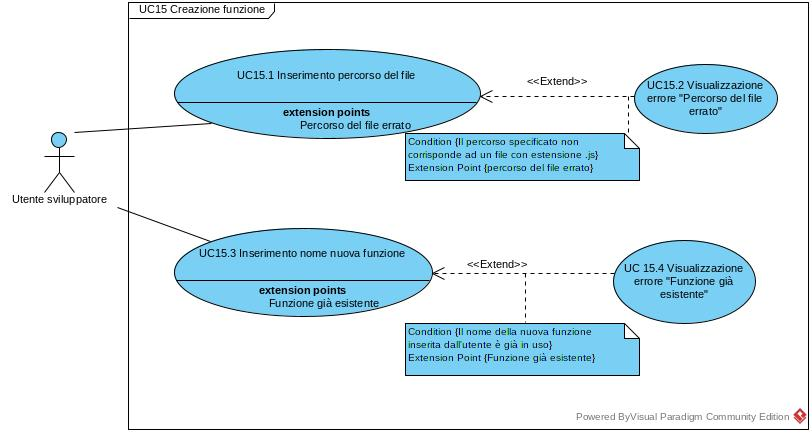
\includegraphics[width=\linewidth]{res/img/UC15.jpg}
	\caption{Diagramma UC16 - Modifica impostazioni funzione}
\end{figure}
\begin{itemize}
	\item \textbf{Attori primari:} Utente sviluppatore;
	\item \textbf{Descrizione:} l'utente potrà modificare alcune impostazioni della funzioni da rendere disponibili agli altri utenti di \textit{Etherless}; 
	\item \textbf{Pre-condizioni:} l'utente ha eseguito il deploy di almeno una funzione su \textit{Etherless};
	\item \textbf{Post-condizioni:} verranno modificate le impostazioni di una determinata funzione e saranno rese visibili agli altri utenti della piattaforma. L'utente visualizzerà a schermo l'esito del comando;
	\item \textbf{Scenario principale:} 
	\begin{enumerate}
		\item L'utente esegue la modifica delle impostazioni di una funzione mediante l'apposito comando. Avrà dunque la possibilità di modificarne:
		\begin{itemize}
			\item costo;
			\item descrizione;
			\item firma.
		\end{itemize}
		\item Il sistema visualizzerà su schermo l'esito dell'operazione effettuata.
	\end{enumerate}
	\item \textbf{Inclusioni:} 
	\begin{itemize}
		\item \textbf{UC18:} l'utente può modificare le impostazioni di una sua funzione solo se già presente in \textit{Etherless}.
	\end{itemize}	
\end{itemize}